% ===============================================================
%  CHAPITRE 2 — RÉSULTATS (~4 pages)
% ===============================================================
\chapter[Résultats]{Ce que montre la simulation}
\label{chap:resultats}

\section{La situation actuelle}
\label{sec:actuel}

Avec le parc actuel, la production locale couvre 41,6~\% de la consommation heure par heure en moyenne, entre 38,4~\% et 44,2~\% selon l'année météo. Ce chiffre est très proche des 42~\% obtenus en volume, et cette proximité est en elle-même un résultat. Elle signifie qu'aujourd'hui la production ne dépasse presque jamais la consommation, puisque le surplus envoyé hors du territoire ne représente que 7~GWh par an, soit 2~\% de la production. Le parc actuel est donc loin de toute saturation. Il reste néanmoins 58,5~\% de l'électricité à acheter au réseau, et jusqu'à 68,5~\% en hiver.

\begin{figure}[H]
\centering
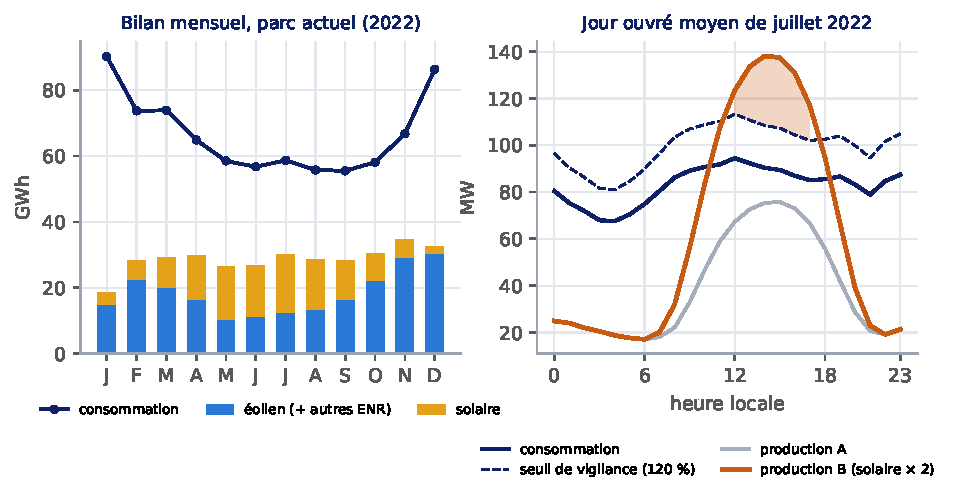
\includegraphics[width=\textwidth]{saisonnalite.pdf}
\caption{Bilan mensuel du parc actuel et jour ouvré moyen de juillet pour les scénarios A et B (2022)}
\label{fig:saison}
\end{figure}

La figure~\ref{fig:saison} explique cette situation. La consommation est maximale en hiver, avec près de 90~GWh en janvier contre 56~GWh en été, sous l'effet du chauffage électrique identifié à la section~\ref{sec:territoire}. L'éolien, qui fournit près des deux tiers de la production, suit heureusement cette saisonnalité. Le solaire produit au contraire l'essentiel de son énergie d'avril à septembre, et toujours autour de midi. C'est cette concentration temporelle qui va limiter son développement.

\section{Les scénarios B et C}
\label{sec:bc}

Le tableau~\ref{tab:scenarios} présente les indicateurs de la fiche pour les trois scénarios. Doubler le solaire augmente la production de 35~\%, mais le taux de couverture ne gagne que 8 points, de 41,6 à 49,5~\%. L'écart entre la couverture en volume et la couverture horaire, quasi nul aujourd'hui, se creuse fortement. Il atteint 7 points en B et 24 points en C, où la production annuelle couvre pourtant 86~\% de la consommation.

\begin{table}[H]
\centering
\footnotesize
\caption{Indicateurs de la fiche pour les trois scénarios, moyenne 2021-2025 et fourchette des cinq années}
\label{tab:scenarios}
{\renewcommand{\arraystretch}{1.2}
\begin{tabularx}{\textwidth}{@{}l>{\centering\arraybackslash}X>{\centering\arraybackslash}X>{\centering\arraybackslash}X@{}}
\toprule
\textbf{Indicateur} & \textbf{A, parc actuel} & \textbf{B, solaire × 2} & \textbf{C, solaire × 3, éolien × 1,5} \\
\midrule
Énergie produite (GWh/an) & 344 & 465 & 694 \\
Production / consommation & 42~\% & 57~\% & 86~\% \\
Taux de couverture horaire & 41,6~\% [38,4 ; 44,2] & 49,5~\% [46,6 ; 51,9] & 61,7~\% [58,8 ; 64,0] \\
Surplus envoyé au réseau (GWh/an) & 7 & 63 & 193 \\
Déficit acheté au réseau (GWh/an) & 475 & 411 & 311 \\
Énergie écrêtée & 0,6~\% [0,2 ; 0,9] & \textcolor{accentOrange}{8,2~\% [5,9 ; 10,3]} & \textcolor{accentOrange}{21,0~\% [18,1 ; 23,7]} \\
Heures de vigilance (h/an) & 165 & 1~236 & 2~363 \\
Pointe d'injection (MW) & 65 & 134 & 241 \\
\bottomrule
\end{tabularx}}
\end{table}

Le jour moyen de juillet de la figure~\ref{fig:saison} montre le mécanisme. En B, la production de midi dépasse le seuil de 120~\% de la consommation pendant environ six heures, et l'énergie située au-dessus de ce seuil doit être écrêtée. L'écrêtement atteint ainsi 8,2~\% de la production en moyenne et dépasse la limite de 5~\% chacune des cinq années, y compris en 2024, la moins ensoleillée. Le scénario C la dépasse largement avec 21~\%. Les heures de vigilance passent de 165 à plus de 2~300 par an, soit plus d'une heure sur quatre. En C, la pointe d'injection de 241~MW dépasse même la pointe de consommation du territoire, qui est de 166~MW. Le réseau local devrait alors évacuer vers l'extérieur une puissance supérieure à tout ce que le territoire peut consommer.

Ces ordres de grandeur sont cohérents entre eux. L'énergie écrêtée en B représente 8,2~\% de 465~GWh, soit environ 38~GWh. Elle est comprise dans les 63~GWh de surplus, qui regroupent toute l'énergie produite au-delà de la consommation, si bien que seuls 25~GWh environ seraient réellement exportés hors du territoire. Le bilan se referme aussi par la consommation, puisque l'énergie couverte localement et le déficit acheté au réseau redonnent bien les 812~GWh consommés. Ni le scénario B ni le scénario C ne respectent donc la règle de la fiche sans flexibilité.

\section{La solution testée, la batterie de la fiche}
\label{sec:batterie}

La fiche impose de tester une batterie dont la capacité correspond à deux heures de la puissance solaire, soit 471~MWh pour le scénario B et 706~MWh pour le scénario C. Techniquement, la batterie remplit son rôle en B. Avec le pilotage qui ne stocke que les excès, l'écrêtement tombe à 0,4~\% en moyenne et ne dépasse jamais 0,8~\%, tandis que la couverture monte à 53,5~\%. En C en revanche, même cette batterie ne suffit pas, puisque l'écrêtement reste de 6,2~\% en moyenne et atteint 8,9~\% la pire année. La figure~\ref{fig:batterie} montre qu'en B, environ 140~MWh suffisent pour respecter la limite de 5~\% chaque année, soit trois fois moins que la taille imposée par la fiche. En C, même 1~060~MWh laissent encore 7,5~\% d'écrêtement la pire année. Elle confirme aussi qu'à taille égale, le pilotage qui réserve la batterie aux excès écrête nettement moins que celui qui stocke tout surplus.

\begin{figure}[H]
\centering
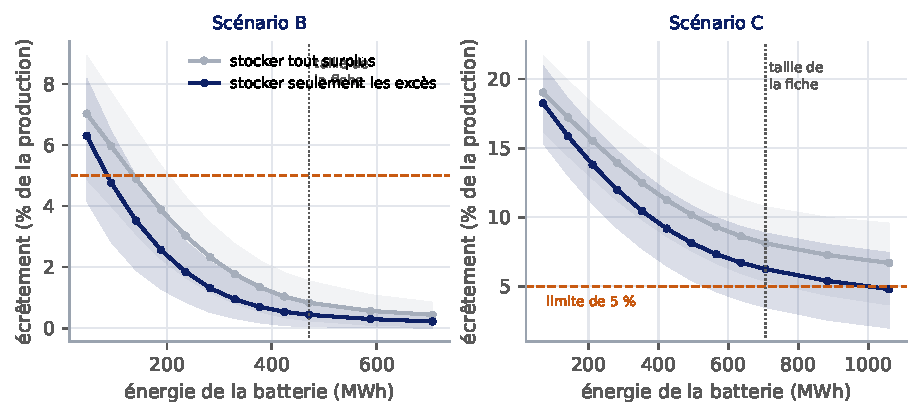
\includegraphics[width=\textwidth]{batterie_taille.pdf}
\caption{Écrêtement en fonction de la taille de la batterie, moyenne et fourchette 2021-2025}
\label{fig:batterie}
\end{figure}

Le coût relatif de cette solution est en revanche rédhibitoire. La batterie du scénario B représente un investissement de 186~M€ et un coût d'exploitation de 11,5~M€ par an. Elle ne fait économiser que 6,4 à 9,7~M€ d'achats d'électricité par an selon le pilotage. Son coût d'exploitation dépasse donc à lui seul le gain qu'elle procure, et sa \gls{van} sur 15 ans vaut entre $-207$ et $-243$~M€. Rapporté au gain de couverture, chaque point supplémentaire coûte environ 46~M€ d'investissement. Une batterie plus petite ne change pas la conclusion. La plus petite capacité qui respecte la limite chaque année, environ 140~MWh, coûterait 56~M€ et rapporterait 3,9~M€ par an pour 3,5~M€ d'exploitation, soit une \gls{van} de $-51$~M€. Nous nous sommes demandé si ce verdict tenait à nos hypothèses de prix. Le tableau~\ref{tab:eco} montre qu'aucune combinaison raisonnable ne rend la batterie rentable, même avec un coût de 250~€/kWh. Valoriser l'électricité évitée au tarif réglementé est d'ailleurs favorable à la batterie, car les industriels, qui consomment plus du tiers de l'électricité du territoire, paient leur électricité bien moins cher que ce tarif résidentiel. Au prix de gros, la \gls{van} se dégrade jusqu'à $-292$~M€. En C, la batterie coûterait 279~M€ sans même rendre le scénario conforme.

\begin{table}[H]
\centering
\footnotesize
\caption{Valeur actuelle nette de la batterie du scénario B (471~MWh) selon les hypothèses économiques}
\label{tab:eco}
{\renewcommand{\arraystretch}{1.2}
\begin{tabularx}{\textwidth}{@{}>{\raggedright\arraybackslash}X cccc@{}}
\toprule
\textbf{Hypothèses} & \textbf{Investissement} & \textbf{Gain annuel} & \textbf{VAN, tout surplus} & \textbf{VAN, excès seuls} \\
\midrule
Base, tarif réglementé 0,194~€/kWh & 186~M€ & 9,7 / 6,4~M€ & $-207$~M€ & $-243$~M€ \\
Prix de gros 0,061~€/kWh & 186~M€ & 2,7 / 2,0~M€ & $-284$~M€ & $-292$~M€ \\
Batterie à 250~€/kWh & 118~M€ & 9,7 / 6,4~M€ & $-91$~M€ & $-128$~M€ \\
Batterie à 500~€/kWh & 235~M€ & 9,7 / 6,4~M€ & $-290$~M€ & $-326$~M€ \\
Hypothèses du projet 6 (10 ans, 5~\%) & 235~M€ & 8,8 / 6,6~M€ & $-167$~M€ & $-184$~M€ \\
\bottomrule
\end{tabularx}}
\end{table}

\section{Les autres leviers et les trajectoires possibles}
\label{sec:leviers}

La batterie n'étant pas une réponse économiquement défendable, nous avons étudié les autres leviers modélisés dans le simulateur. Le plus efficace est le déplacement de la chauffe des ballons d'eau chaude. Faute de statistique locale sur l'eau chaude, nous avons supposé qu'environ la moitié des résidences principales recensées par l'\gls{insee}, soit 26~000 logements, dispose d'un ballon électrique, ce qui correspond à l'ordre de grandeur national d'une quinzaine de millions de chauffe-eau pour 30 millions de résidences principales~\cite{construction21}. Ces ballons représentent 58~MW de puissance et 26~GWh par an. Les chauffer entre 10~h et 17~h plutôt que la nuit permet d'absorber une partie du surplus solaire sans aucun équipement lourd, et la réforme des heures creuses engagée par la \gls{cre}, qui place des heures creuses l'après-midi en été, va déjà dans ce sens~\cite{cre_hphc}. Dans le scénario finalement recommandé, ce levier fait passer l'écrêtement de 4,0 à 3,2~\% et celui de la pire année de 5,0 à 4,1~\%, ce qui fait sortir la trajectoire de la zone limite. Ce levier concerne cependant directement les ménages, et sa mise en œuvre suppose un signal tarifaire ou un pilotage accepté par les habitants. Le pilotage de la recharge des \gls{ve} n'a d'effet qu'à l'horizon 2035, lorsque le parc atteindrait environ 30~600 véhicules. Même en déplaçant à midi l'ensemble des recharges pilotables, le gain de couverture ne dépasse pas 0,4 point. Le plafond d'injection, enfin, réduit l'écrêtement en limitant la puissance des onduleurs, mais il perd l'énergie au lieu de la déplacer.

Pour savoir jusqu'où aller sans stockage, nous avons simulé 360 combinaisons de puissances solaire et éolienne, de leviers et d'horizons. La figure~\ref{fig:trajectoires} présente le cas avec les ballons pilotés. Elle met en évidence une concurrence entre l'éolien et le solaire. Plus on ajoute d'éolien, moins il reste de place pour le solaire sous la limite de 5~\%. Avec 75~\% d'éolien en plus, le parc solaire actuel dépasse déjà la limite certaines années. Le taux de couverture maximal atteignable sans stockage se situe autour de 55 à 57~\%, obtenu avec 50~\% d'éolien en plus et entre 25 et 40~\% de solaire en plus.

\begin{figure}[H]
\centering
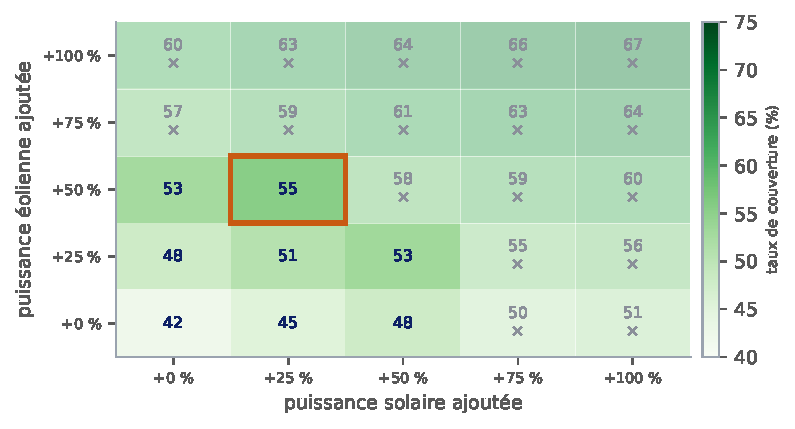
\includegraphics[width=0.8\textwidth]{trajectoires.pdf}
\caption{Taux de couverture moyen selon la puissance ajoutée, avec les ballons pilotés. Les croix signalent un écrêtement supérieur à 5~\% au moins une année, le cadre orange le scénario recommandé}
\label{fig:trajectoires}
\end{figure}

Ces conclusions résistent-elles aux incertitudes du modèle~? Une analyse de sensibilité, qui fait varier une à une les principales hypothèses entre une valeur basse et une valeur haute, montre que l'année météo reste le facteur le plus influent, devant la taille et le pilotage de la batterie. La forme du profil de consommation et le rendement de la batterie n'ont en revanche qu'un effet marginal. Les conclusions ne reposent donc pas sur les choix de reconstruction les plus incertains. À l'horizon 2035 enfin, l'électrification des usages porterait la consommation de 812 à 904~GWh. La couverture du parc actuel baisserait de 41,6 à 37,4~\%, mais l'écrêtement diminuerait aussi, puisque la consommation supplémentaire absorberait une partie des surplus.
